\chapter{Grundlagen}

\section{Einführung}
	Entwurf einer Rechneranlage: Ingenieurmäßige Aufgabe der Kompromissfindung zwischen Zielsetzung, Randbedingungen, Gestaltungsgrundsätzen und Anforderungen.

\section{Entwurf von Rechneranlagen - Entwurfsfragen}
	\paragraph{Heutige Kennzahlen}
		\begin{itemize}
			\item Höchstleistungsrechner: Exa-FLOPs ($10^{18}$)
			\item Intel Skylake-Prozessoren: 8 Mrd. Transistoren
			\item Strukturbreite: 10nm 
		\end{itemize}

	\paragraph{Prozessortypen}
		\begin{itemize}
			\item Multicore/Manycore
			\item Anwendungsspezifisch, bspw. Google TPUs 
		\end{itemize}

	\paragraph{Zielsetzung}
		\begin{itemize}
			\item \textbf{Einsatzgebiet}
			\begin{itemize}
				\item \textbf{Desktop Computing}
				\begin{itemize}
					\item PCs bis Workstations (\$1000 - \$10.000)
					\item Günstiges Preis-/Leistungsverhältnis
					\item Ausgewogene Rechenleistung für ein breites Spektrum von (interaktiven) Anwendungen
				\end{itemize}
				\item \textbf{Server}
				\begin{itemize}
					\item Rechen- und datenintensive Anwendungen
					\item Hohe Anforderungen an die Verfügbarkeit und Zuverlässigkeit
					\item Skalierbarkeit
					\item Große Dateisysteme und Ein-/Ausgabesysteme
				\end{itemize}
				\item \textbf{Eingebettete Systeme}
				\begin{itemize}
					\item Mikroprozessorsysteme, eingebettet in Geräte und daher nicht unbedingt sichtbar
					\item Sind auf spezielle Aufgaben zugeschnitten (hohe Leistungsfähigkeit, Spezialprozessoren)
					\item Breites Preis-/Leistungsspektrum
					\item Echtzeitanforderungen
					\item Abwägung der Anforderungen an Rechenleistung, Speicherbedarf, Kosten, Energieverbrauch, etc.
				\end{itemize}
			\end{itemize}
			\item \textbf{Anwendungsbereich}
			\begin{itemize}
				\item Technisch-wissenschaftlicher Bereich: Hohe Anforderungen an die Rechenleistung, insbesondere Gleitkommaverarbeitung
				\item Kommerzieller Bereich: Datenbanken, WEB, Suchmaschinen, Optimierung von Geschäftsprozessen, etc.
				\item Eingebettete Systeme: Verarbeitung digitaler Medien, Automatisierung, Telekommunikation, etc.
			\end{itemize}
			\item \textbf{Rechenleistung}
			\begin{itemize}
				\item Ermittlung über Benchmarks
				\item Maßzahlen für die Operationsleistung: \textit{MIPS} oder \textit{MFLOPS}
				\item \(MFLOPS = \frac{\texttt{Anzahl ausgeführter Gleitkommainstruktionen}}{10^6 \cdot \texttt{Ausführungszeit}}\)
			\end{itemize}
			\item Verfügbarkeit
			\item \textbf{Zuverlässigkeit}
			\begin{itemize}
				\item Bei Ausfällen von Komponenten muss ein betriebsfähiger Kern bereit sein
				\item Verwendung redundanter Komponenten
				\item Bewertung der Ausfallwahrscheinlichkeit mittels stochastischer Verfahren
				\item Definition Verfügbarkeit: Wahrscheinlichkeit, ein System zu einem beliebigen Zeitpunkt fehlerfrei anzutreffen
			\end{itemize}
		\end{itemize}

	\paragraph{Randbedingungen}
		\begin{itemize}
			\item Technologische Entwicklung: Mikrominiaturisierung setzt sich fort, beispielsweise Verkleinerung der Strukturbreiten sowie Erhöhung der Integrationsdichte (Anzahl der Transistoren verdoppelt sich alle 18 Monate)
			\item Größe
			\item Geld
			\item \textbf{Energieverbrauch}
			\begin{itemize}
				\item Mobile Geräte: Verfügbare Energiemenge durch Batterien und Akkumulatoren ist begrenzt \(\rightarrow\) möglichst lange mit der vorhandenen Energie auskommen
				\item Vermeiden von Überhitzungen
				\item Green IT: Niedriger Energieverbrauch, ökologische Produktion, einfaches Recycling
			\end{itemize}
			\item Umwelt
		\end{itemize}

	\paragraph{Sonstiges}
		\begin{itemize}
			\item Gestaltungsgrundsätze: Modularität, Sparsamkeit, Fehlertoleranz, etc.
			\item Anforderungen: Kompatibilität, Betriebssystemanforderungen, Standards, etc.
		\end{itemize}

\paragraph{Trends in der Rechnerarchitektur: Herausforderungen}
Weltweite Forschungsaktivitäten bzgl. ExaScale-Rechner
\begin{itemize}
	\item Verlustleistung: Überträgt man heutige (Stand 2010) Höchstleistungsrechner in den Exascale-Bereich, hätte man eine Verlustleistung von etwa 40 GW (diese kann allerdings höchstens 20-40 MW betragen)
	\item Hauptspeicher (DRAM), permanenter Speicher: Kapazität und Zugriffsgeschwindigkeit muss mit der Rechengeschwindigkeit mithalten
	\item Zuverlässigkeit und Verfügbarkeit
	\item Parallelität und Lokalität
\end{itemize}


\section{Effizienter Entwurf --- Grundlagen}
	\begin{itemize}
		\item Mobile Geräte: Verfügbare Energiemenge durch Batterien und Akkus begrenzt \(\rightarrow\) vorhandene Energie möglichst lange ausnutzen sowie Vermeidung von Überhitzung
		\item HPC: Hohe Temperaturen begrenzen die Verarbeitungsgeschwindigkeit und die beeinflussen die Zuverlässigkeit
	\end{itemize}

	\paragraph{CMOS-Schaltung}
		\begin{itemize}
			\item MOSFET: Je nach Spannung am Gate und dem daraus resultierenden Feld im Kanal können Ladungsträger den Kanal passieren oder nicht. Extrem niedrige Stromaufnahme im Ruhezustand
			\item \textbf{Leistungsaufnahme}
			\begin{itemize}
				\item \(P_{total} = P_{switching} + P_{shortcircuit} + P_{static} + P_{leakage}\)
				\item Statischer Leistungsverbrauch: \(P_{static}\) sowie Leistungsverbauch $(P_{leakage}$ bei Kriechströmen
				\item Verbrauch bei Zustandsänderung: \(P_{switching}=C_{eff}*V_{dd}^2*f\) sowie Verbrauch während des Übergangs am Ausgang, wenn sich die Eingänge ändern \(P_{shortciruit}=I_{mean}*V_{dd}\) 
				\item Höhere Frequenzen erfordern steilere Taktflaken \(\rightarrow\) schnelleres Laden von \(C_{eff}\) \(\rightarrow\) höhere Versorgungsspannung 
				\item \(P \sim f und P \sim V_{dd}^2\) aber da $f \sim V_{dd}^2 \Rightarrow P \sim V_{dd}^3 $ und $P \sim f^3$
				\item Energieverbrauch pro Aufgabe ist unabhängig von Frequenz, bzw. sogar negativ korreliert wegen statischer Ströme		
			\end{itemize}
			\item \textbf{Schaltwahrscheinlichkeit}
			\begin{itemize}
				\item \(\mathbb{P}_{Schalt} = 2 \cdot \mathbb{P}_{Ausgang(1)} \cdot (1-\mathbb{P}_{Ausgang}(1))\)
				\item \(\mathbb{P}_{Ausgang}(1) = \mathbb{P}_{Eingang1}(0) \cdot \mathbb{P}_{Eingang2}(1) + \mathbb{P}_{Eingang1}(1) \cdot \mathbb{P}_{Eingang2}(0)\)
			\end{itemize}
	\end{itemize}

	\paragraph{Kosten von Prozessoren}
		\begin{itemize}
			\item \textbf{Ziel}
			\begin{itemize}
				\item Leistungsaufnahme senken ohne Verarbeitungsgeschwindigkeit zu beeinträchtigen
				\item Optimierung der Systemarchitektur
				\item Spezialisierte Prozessorkerne/Multicore-CPUs, die Parallelverarbeitung erlauben, verwenden
			\end{itemize}
			\item \textbf{Kosten} Proportional zu $\sqrt{A_{Wafer}}$, Chipfläche wird durch Entwickler beeinflusst
			\begin{itemize}
				\item $C_{Die}=\frac{C_{Wafer}}{\frac{\texttt{\#Dies}}{Wafer}*Ausbeute}$
				\item $\texttt{\#Dies}=\frac{\pi*r_{Wafer}^2}{A_{Die}}-\frac{2\pi*r_{Wafer}}{\sqrt{2*A_{Die}}}$
				\item $\texttt{Ausbeute}=\frac{\texttt{Ausbeute}_{Wafer}}{(1+\texttt{Defekte})^N}$
			\end{itemize}
		\end{itemize}

\section{Einführung in den Entwurf eingebetteter Systeme}
	\paragraph{Die Hardware-Beschreibungssprache VHDL}
		\begin{itemize}
			\item Standardisierte Hardware-Beschreibungssprache: Die verschiedenen Schaltungsbeschreibungen des gesamten Entwurfsablaufs können dargestellt werden - von der algorithmischen Spezifikation bis hin zu realisierungsnahen Strukturen
			\item Eingesetzt zum ASIC- und FPGA-Entwurf
			\item Bei synchroner Zuweisung werden Änderungen abhängig von einem Takt und den Eingangssignalen geändert. Bei asynchroner Zuweisung unabhängig und unmittelbar (nach einer gewissen Schaltzeit)
			\item Automatischer Synthesewerkzeuge: Flexibilität, weniger fehleranfällig. Dafür Randbedingungen schwer einzuhalten und Ergebnisse oft schlechter als bei manuellem Entwurf
		\end{itemize}
	\paragraph{Chip-Entwurf(Top-Down)}
		\begin{itemize}
			\item Grundlage des Entwurfs ist die Spezifikation der Schaltung: Gewünschtes Verhalten; Schnittstellen; Vorgaben bzwgl. Geschwindigkeit, Kosten, Fläche oder Leistungsverbrauch
			\item Entwurfsschritte: Verhaltensspezifikation, High-Level-Synthese, RT-Beschreibung, Logik-Synthese, Gatterbeschreibung, Layout-Synthese, Geometriegebschreibung, Fertigung
			\item \textbf{Hauptbestandteile} 
			\begin{itemize}
				\item ENTITY: Schnittstellen
				\item ARCHITECTURE: Verhalten
				\item CONFIGURATION: Weist COMPONENT-Instanzen zu ENTITY und ARCHITECTURE zu.
			\end{itemize} 
			\item Signale zur Kommunikation zwischen Instanzen untereinander oder mit Schnittstellen der äußeren Hülle (Entity)
			\item Schnittstellendefinition eines MODULS\\\\
			\begin{minipage}{\linewidth}
				\begin{lstlisting}[frame=single,numbers=left,mathescape,language=VHDL,tabsize=4]
	ENTITY blinklicht IS
		PORT(
			clk: IN Std_Logic;
			reset: IN Std_Logic;
			led: OUT Std_Logic
		);
	END blicklicht
				\end{lstlisting}
			\end{minipage}
			\item Schema einer ARCHITECTURE\\\\
			\begin{minipage}{\linewidth}
				\begin{lstlisting}[frame=single,numbers=left,mathescape,language=VHDL,tabsize=4]
	ARCHITECTURE Structure OF blinklicht IS
		COMPONENT Counter
		GENERIC(countMax : positive);
		PORT(
			clk: IN Std_Logic;
			out: OUT Std_Logic
		);
		END COMPONENT
		COMPONENT DCM
		PORT(
			clkin_in: IN Std_Logic;
			rst_in: Std_Logic;
			clkdv_out: OUT Std_Logic
		);
		END COMPONENT

		Signal clk_int: Std_Logic

		BEGIN
			Inst:DCM: DCM
			PORT MAP(
				clkin_in => clk,
				rst_in => reset,
				clkdv_out => clk_int,
			);
			Inst_counter: counter
			GENERIC MAP (countMax => 25000000)
			PORT MAP(
				clk => clkIn,
				out => led
			);
		END Structure
				\end{lstlisting}
			\end{minipage}
		\end{itemize}


\section{Bewertung der Leistungsfähigkeit eines Rechners}
	\paragraph{Definitionen}
		\begin{itemize}
			\item Wall-clock time, response time, elapsed time: Globale Latenzzeit für die Ausführung einer Aufgabe
			\item CPU time (Vgl Unix time Kommando)
			\begin{itemize}
				\item CPU time: Zeit, in der die CPU arbeitet
				\item User CPU time: Zeit, inder die CPU ein Programm ausführt
				\item System CPU time: Zeit, in der die CPU Betriebssystemaufgaben ausführt, die von einem Programm angefordert werden
			\end{itemize}
		\end{itemize}

	\paragraph{Einfache Hardwaremaße}
		\begin{itemize}
			\item Clock cycles per instruction: \(CPI = \frac{\text{CPU time}}{\text{instruction count } \cdot \text{ machine cycle time}} = \frac{T_{exe}}{IC \cdot T_C}\)
			\item Instructions per cycle: \(IPC = \frac{1}{CPI}\)
			\item Millions of instructions per second: \(MIPS = \frac{\texttt{Anzahl der ausgeführten Instruktionen}}{10^6 \texttt{ Ausführungszeit}}\), Floatingpointoperationen (MFLOPS) analog. Niedrigere MIPS-Werte resultieren bei gleicher Laufzeit in kompakterem Code, niedrigerer Schaltfrequenz und damit geringerem Energieverbrauch
			\item Probleme: Angaben meist theoretische Maximalwerte bzw. abhängig vom konkreten Programm 
		\end{itemize}

	\paragraph{Laufzeitmessungen bestehender Programme}
		\begin{itemize}
			\item Bewertung der Leistungsfähigkeit mit Hilfe von einem Programm oder einer Programmsammlung und Messen der Ausführungszeit. Problem: Zugriff auf die Maschine notwendig und abhängig von der Güte des Compilers
			\item Kernels: Rechenintensive Teile reale Programme, vorwiegend numerische Algorithmen (beispielsweise LINPACK Softwarepaket zum Lösen linearer Gleichungen)
			\item \textbf{Standardisierung}
			\begin{itemize}
				\item Zur Verbesserung der Vergleichbarkeit von Rechnern (inklusive OS und Compiler), z.B. SPEC CPU Benchmarks
				\item SPEC: Non-profit Organisation, die Benchmarks zur Leistungsbewertung von Hardware und Software entwickelt. Mit dem Erwerb einer Lizenz verpflichten sich die jeweiligen Unternehmen, immer die kompletten Ergebnisse zu veröffentlichen. \footnote{\url{https://de.wikipedia.org/wiki/Standard_Performance_Evaluation_Corporation}}
				\item $SPEC_{ratio} = \frac{\texttt{Referenzzeit}_x}{\texttt{Laufzeit}_x\texttt{ auf Testsystem}}$ für Benchmark $x$. Der Endwert wird als geometrisches Mittel über alle Benchmarks berechnet, aufgrund der normalisierung unabhängig von der Referenzmaschine.
			\end{itemize}
		\end{itemize}

	\paragraph{Messung während des Betriebs von Anlagen}
		\begin{itemize}
			\item Monitore: Aufzeichnungselemente, welche die Verkehrsverhältnisse während des normalen Betriebs beobachten oder untersuchen
			\item Hardware-Monitor: Unabhängige physikalische Geräte, welche die Betriebsverhältnisse nicht beeinflussen
			\item Software-Monitor: Eingebaut ins OS, beeinträchtigen die normalen Betriebsverhältnisse
			\item Aufzeichnungstechniken: Kontinuierlich/spärlich, Gesamttracing, Realzeitauswertung, Post Processing 
			\item Beispiel: Performance Counter
			\begin{itemize}
				\item Misst verschiedene geschwindigkeitsrelevante Vorgänge, die ein Prozessor ausführt. Dabei beeinträchtigt er die Abarbeitung anderer Aufgaben im Prozessor nicht. Heutige Prozessoren erreichen bei den aktuellen Prozessortakten eine Auflösung im Mikro- bis Nanosekundenbereich\footnote{\url{https://de.wikipedia.org/wiki/Performance_Counter_(Mikroprozessor)}}
				\item Metriken zur Darstellung bestimmter Messgrößen. Beispielsweise Anzahl ausgeführter Befehle, Cache-Treffer oder Fehlzugriffe
			\end{itemize}
		\end{itemize}

	\paragraph{Modelltheoretische Verfahren}
		\begin{itemize}
		\item Unabhängig von Existenz eines Rechners
		\item Modellbildung: Annahmen über die Struktur und Betrieb eines Rechners sowie Analyse der relevanten Merkmale des Systems 
		\item Ziel: Beziehungen zwischen Systemparametern aufdecken und Leistungsgrößen ermitteln
		\item Stellt für Analyse relevante Systemkomponenten und deren Datenverkehr dar
		\item \textbf{Analytische Methoden}
			\begin{itemize}
				\item Versucht mathematische Beziehungen zwischen Leistungsgrößen herzuleiten. Oft minimaler Aufwand aber auch nur minimal aussagekräftig (beispielsweise Warteschlangenmodelle, Petrinetze, Diagnosegraphen, Netzwerkflussmodelle)
				\item Gesetz von Little: Für ein stabiles Warteschlangensystem gilt \[k=\lambda t\] mit $k$ als durchschnittliche Anzahl an Kunden im System, $\lambda$ als durchschnittliche Ankunftsrate und $t$ als durchschnittlicher Verweildauer.
			\end{itemize}
		\item \textbf{Simulationen}
			\begin{itemize}
				\item Modellierung zur evaluation neuer Ideen und der Exploration des Entwurfsraums. Mögliche Zielgrößen: Rechenleistung, Leistungsaufnahme, Zuverlässigkeit
				\item Kompromiss zwischen Genauigkeit, kosten, Flexibilität und Komplexität
				\item Taxonomie
				\begin{itemize}
					\item User-Level Simulatoren: Simulation der Mikroarchitektur eines Prozessors ohne Berücksichtigung von Systemressourcen
					\item Full-System Simulatoren modellieren ein vollständiges Computersystem, einschließlich CPU, IO, Disk und Netzwerk	
					\item Functional Simulatoren modellieren nur Funktionalitöt eines Prozessors, aber keine Berücksichtigung der Mikroarchitektur
					\item Cycle-accurate Simulatoren erfassen parametrisierbare Details von Mikroarchitekturblöcken um Funktionalität und Zeitverhalten zu emulieren
				\end{itemize}
				\item Prozessimulatoren benötigen Liste von Befehlen die ausgeführt werden müssen
				\begin{itemize}
					\item Trace-driven Simulation: Durchführung des Benchmarks auf anderem Prozessor/ Simulator, dabei die Befehle \emph{tracen}. Diese Trace kann dann für einen Zyklengenauen Simulator verwendet werden. Jede Instruktion wird aud Basis des Mikroarchitekturmodells simuliert
					\item Execution-driven Simulation: Simulator muss Zeitverhalten und Funktionalität genau reproduzieren. Daher aufwendig in der Entwicklung aber dafür genauer und flexibler
				\end{itemize} 
			\end{itemize}
		\end{itemize}


\section{Zuverlässigkeit und Fehlertoleranz}
	\paragraph{Definitionen}
		\begin{itemize}
			\item Zuverlässigkeit: Wird während gewisser Zeitdauer bei zulässigen Betriebsbedingungen die spezifizierte Funktion erbracht?
			\item Fehlertoleranz: Ist das System trotz begrenzter Anzahl fehlerhafter Subsysteme in der Lage die spezifizierte Funktion zu erbringen?
			\item Sicherheit: Nichtvorhandensein einer Gefahr unter anzunehmenden Betriebsbedingungen. Verfügbarkeit, Überlebenswahrscheinlichkeit, ...
			\item Vertraulichkeit: Datenschutz und Zugangssicherheit
		\end{itemize}

	\paragraph{Fehler}
		\begin{itemize}
			\item \textbf{Zustände}
			\begin{itemize}
				\item Fehlerfrei, sicher
				\item Fehlerhaft, sicher/in Gefahr
				\item Schaden/ Funktionsausfall
			\end{itemize}
			\item \textbf{Ursachen}
			\begin{itemize}
				\item Entwurf (Spezifikation/Implementierung/Dokumentation)
				\item Herstellung
				\item Betrieb: Störung (externer Einfluss), Verschleiß, zufällig physikalischer Fehler, Bedienung,  Wartung
			\end{itemize}
			\item Dauer: Temporär oder Permanent
		\end{itemize}

	\paragraph{Struktur-Funktions-Modell}
		\begin{itemize}
			\item Gerichteter Graph, dessen Knoten die Komponenten und dessen Kanten die Funktionen eines Systems repräsentieren. Eine Kante \(K_i \longrightarrow K_j\) bedeutet, dass \(K_i\) eine Funktion erbringt, die von \(K_j\) genutzt wird
			\item eine Komponentenmenge ist ein System, wenn die erbrachten Funktionen durch eine äußere Spezifikation festgelegt werden		
			\begin{figure}
				\begin{center}
					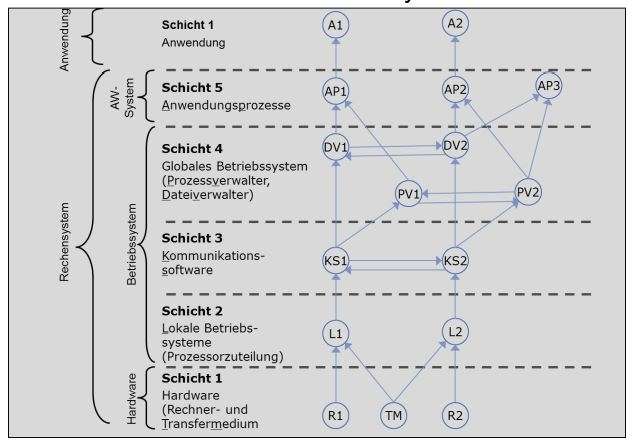
\includegraphics[width=0.4\textwidth]{assets/schichtenmodell.jpg}
					\caption{Schichtenmodell eines Zweirechensystems. Funktionszuordnungen sind nur von unteren auf höhere Schichten möglich.}		
				\end{center}
				\end{figure}	
			\item Binäres Fehlermodell gibt für jede Komponente und das Gesamtsystem an ob sie fehlerfrei sind: $Z: (S \cup \{S\}) \rightarrow \{\texttt{wahr, falsch}\}$. Die Systemfunktion gibt in Abhängigkeit der Komponenten die Funktion des Systems an.
			\item Zuverlässigkeitsblockdiagramm: Zeigt mögliche "`Verbindungspfade"' zwischen den Komponenten, von denen mindestens einer in Takt sein muss. Reihenschaltung von AND-Bausteinen, Parallelschaltung von OR-Bausteinen. Äquivalent zur Systemfunktion.
			\item Negierter Systemfunktionsbaum (alle Blätter werden negiert, alle Verknüpfungen werden vertauscht (\(AND \leftrightarrow OR\))) gibt an, wie sich Fehler des Systems auf Fehler der Komponenten zurückführen lassen.
			\item \textbf{Fehlerbereiche} 
			\begin{itemize}
				\item Komponenten, welche zeitgleich fehlerhaft sein können ohne zu Systemfehlern zu führen. 
				\item Einzelfehlerbereich: Menge von Komponenten, die exakt denselben Fehlerbereichen angehören
				\item Perfektionskern: Das Komplement der Vereinigung aller Fehlerbereiche $\rightarrow$ Komponenten, welche nicht ausfallen dürfen
			\end{itemize}
		\end{itemize}

	\paragraph{Ausfallverhalten}
		\begin{itemize}
			\item Teilausfall: Es fallen nicht alle Funktionen aus
			\item Unterlassungsausfall (Fail-silent-System): Keine Ausgabe fehlerhafter Ergebnisse. Wenn ein Ergebnis ausgegeben wird, ist es korrekt
			\item Anhalteausfall (Fail-stop-System): Keinerlei Ergebnisausgabe mehr
			\item Haftausfall: Komponente gibt ständig denselben Ergebniswert aus
			\item Binärstellenausfall: Ein Fehler verfälscht eine/mehrere Binärstellen
			\item Unkritische Ausfälle (Fail-safe-System)
		\end{itemize}

	\paragraph{Fehlereingrenzung}
		\begin{itemize}
				\item Vertikal: Niedrigere Schichten prüfen Funktionsaufrufe vor Ausführung, Fehlerkorrekturcode in der Hardware, Plausibilitäts-/Konsistenzprüfungen
				\item Horizontal: Isolierung fehlerhafter lokaler Knoten. Problem vor allem bei globalen Schichten.		 
		\end{itemize}
		
	\paragraph{Zuverlässigkeit}
		\begin{itemize}
			\item Um Anforderungen zu erfüllen sind Fehlertoleranz (Redundanz) und Fehlervermeidung wichtig. Zuverlässigkeitskenngrößen können als Verteilungsfunktionen von Lebensdauer, Fehlerbehandlungsdauer und Sicherheit statistisch betrachtet werden:
			\begin{itemize}
				\item $F_L(t)=\frac{N_f(t)}{N}=\frac{N-N_s(t)}{N}=1-R(t)=1-e^{-\lambda t}$ - Wahrscheinlichkeit, dass ein funktionierende System fehlerhaft wird mit Anzahl Komponenten $N$ und $f$ failed oder $s$ survived. Fehlerwarscheinlichkeit exponentialverteilt mit Parameter $\lambda$
				\item $R(t)=\frac{N_s(t)}{N}$ - Überlebenswahrscheinlichkeit
				\item $N_f(t)=N-N_s(t)$
				\item $z(t)=\frac{f_L(t)}{R(t)}$ als Ausfallrate
				\item Ausfallverhalten ("`Badewannenkurve"'): Frühphase (hohe Ausfallwahrscheinlichkeit durch Fertigungsfehler oder defekte Bauteile), Betriebsphase, Spätphase (hohe Ausfallwahrscheinlichkeit durch Verschleiß)
				\item $V=\frac{E(L)}{E(L)+E(B)}$ als Verfügbarkeit mit Lebensdauer $L$ und Behandlungsdauer $B$
				\item $\phi(S)=\sum_{(K_1,\dots,K_n)\in f^{-1}(\texttt{wahr})}\phi(\wedge_{i=1}^n K_i) $ Funktionswahrscheinlichkeit
				\item Weitere Kenngrößen: Gefährdungwahrscheinlichkeit, Sicherheitswahrscheinlichkeit, mittlere Sicherheitsdauer
			\end{itemize}
		\end{itemize}

	\paragraph{Redundanz}
		\begin{itemize}
			\item Statische Redundanz: Vorhandensein redundanter Systeme während des gesamten Einsatzzeitraums (n-von-m-System)
			\item Statische Redundanz/Zuverlässigkeit von n-von-m-Systemen (3-aus-5 vs. 2-aus-3): Das 3-aus-5-System zeigt in der Anfangszeit eine höhere Funktionswahrscheinlichkeit als das 2-aus-3-System. Nach einiger Zeit (Schnittpunkt der beiden Graphen im Bild) kehrt sich dieser Effekt jedoch um. Anfangs sind die einzelnen Funktionswahrscheinlichkeiten noch hoch und bei einem 3-aus-5-System können bis zu 2 Komponenten ausfallen. Wenn die Funktionswahrscheinlichkeit einen bestimmten Punkt unterschreitet, ist ein 2-aus-3-System sicherer, da nur 2 Komponenten zum Betrieb notwendig sind
			\item Dynamische Redundanz: Vorhandensein redundanter Systeme, die erst nach Auftreten eines Fehlers aktiviert werden. Kann zuvor ungenutzt oder fremdgenutzt sein. Auch gegenseitige Redundanz möglich.
		\end{itemize}


\section{Grundlagen der Parallelverarbeitung}
	\paragraph{Formen} 
		\begin{itemize}
			\item Nebenläufigkeit: Objekte werden vollständig gleichzeitig abgearbeitet
			\item Pipelining: Bearbeitung von Objekten wird in sequentielle Teilschritte zerlegt. Pipelinephasen dürfen für verschiedene Objekte überlappen.	
		\end{itemize}

	\paragraph{Ebenen}
		\begin{itemize}
			\item Programmebene: Vom OS organisisert, vollständig unabhängige Einheiten die parallel verarbeitet werden
			\item Prozess/Taskebene: Programm wird in parallel ausführbare Prozesse zerlegt, jeweils eigener Adressraum. Benötigt Synchronisation und Kommunikation, Primitive durch OS implementiert
			\item Blockebene: Threads, teilen sich Adressraum, Synchronisation über Mutex usw., dafür geringerer Aufwand für Erzeugung/ Beendigung/ Wechsel im Vergleich zum Prozess
			\item Anweisungs-/Befehlsebene: Parallele Ausführung elementarer Anweisungen, Optimierende Compiler, Umordnen und Parallelisieren von Befehlen, Superskalar-Technologie
			\item Suboperationsebene: Aufbrechen elementarer Anweisungen in parallel auszuführende Suboperationen durch Compiler, bspw. überlappte Ausführung bei Vektorrechner in Vektorpipeline
		\end{itemize}
		Körnigkeit der Parallelität: Verhältnis Rechenaufwand zu Synchronisationsaufwand.

\section{Klassifikation von Rechnerarchitekturen}
	\paragraph{Flynn'sche Taxonomie} 
		\begin{itemize}
			\item Zahl-, Befehls- und Datenströme
			\item Single Instruction, Single Data (SISD): Uniprozessor
			\item Single Instruction, Multiple Data (SIMD): Vektorrechner, Feldrechner
			\item Multiple Instruction, Single Data (MISD): Zuordnung Umstritten ("`darf es nicht geben"' vs. "`Großrechner oder Supercomputer"')
			\item Multiple Instruction, Multiple Data (MIMD): Multiprozessor
		\end{itemize}